% !TeX root = thesis.tex
\documentclass{master_thesis}
\addbibresource{refs.bib}

\begin{document}

\section{Results}

% This section should have answers to all my research questions
% Follow up survey + reach out to devs I know have used addon-a11y

\subsection{Comparing results from manual audit and automated report}

To get the whole list including all components a report was created that included the violations caught in each example of each component. This report was generated at the beginning of the manual audit, so the results obtained from both methods are based on the same source code.
\begin{figure}[H]
	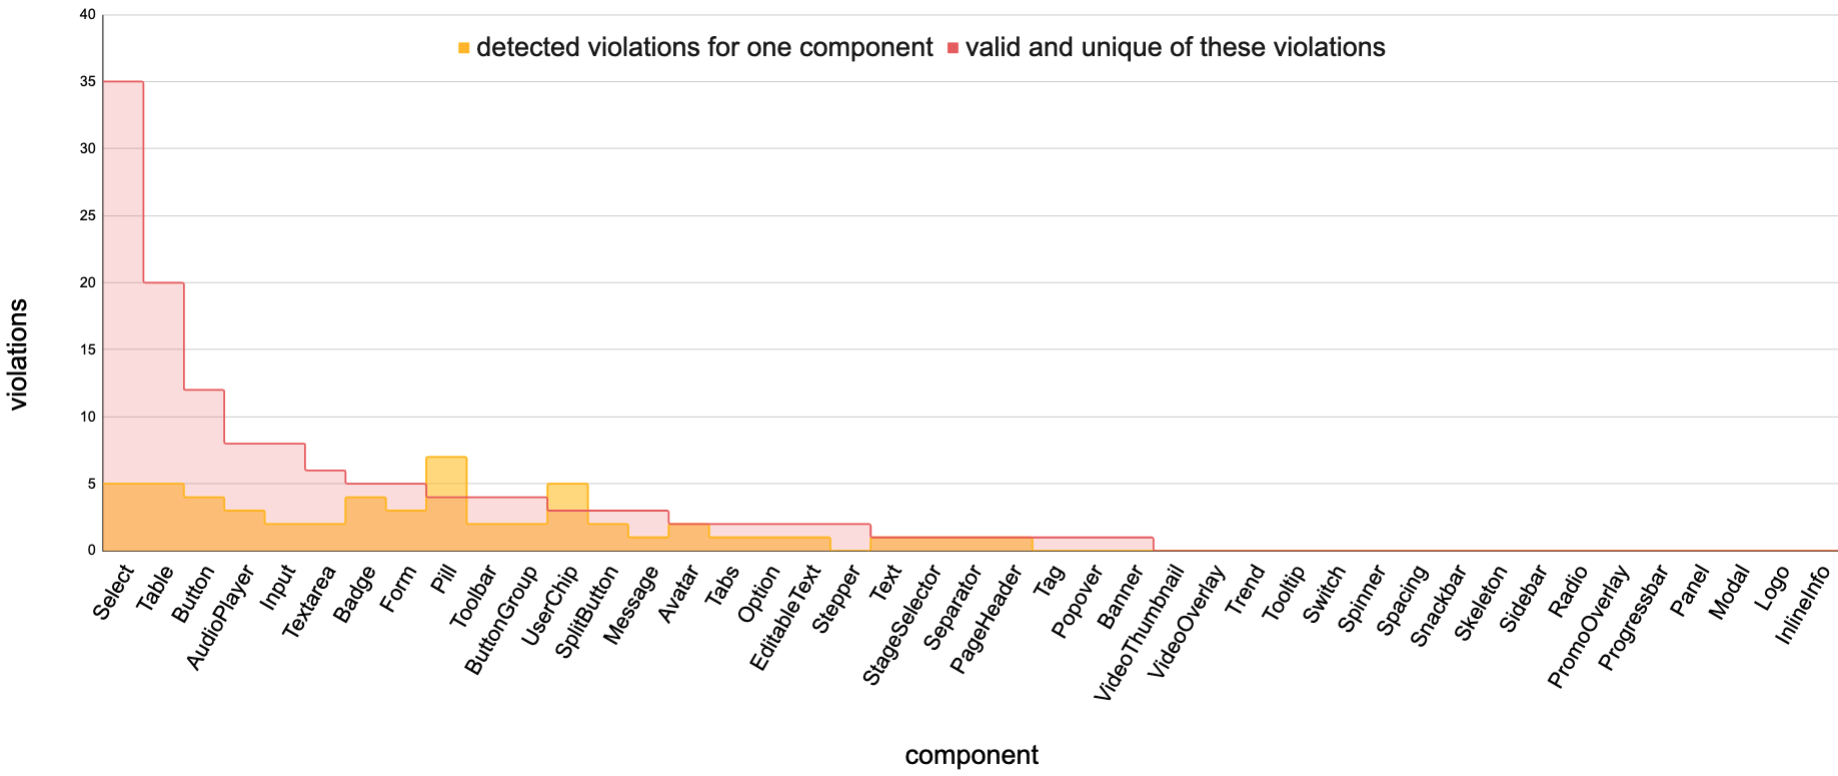
\includegraphics[width=\textwidth]{img/audit-failed.png}
	\caption{All violations found by addon-a11y and how many of them are valid.}
	\label{fig:audit-failed}
\end{figure}

I prepared a comparison table from both results. For automated accessibility tests, I recorded the number of examples that included violations, the number of different violations and the number of passed checks for each component. In most cases, there were more examples with violations because the same thing was reported in more than one example (see figure \ref{fig:audit-failed}). Addon-a11y did not report any issues for 27 components out of 53 components.

\begin{figure}[H]
	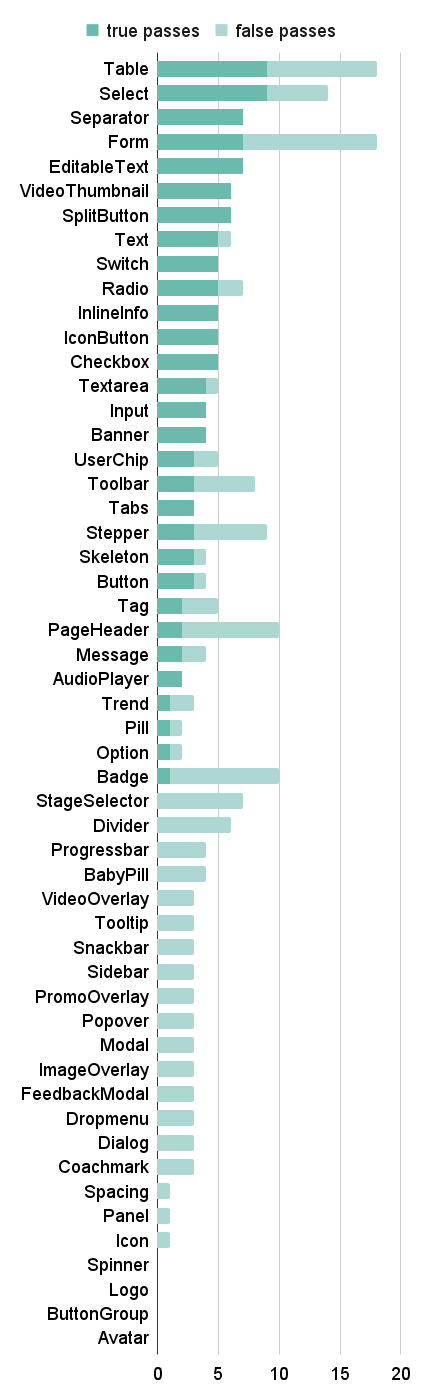
\includegraphics[width=\textwidth]{img/audit-passed.png}
	\caption{All passed checks reported by addon-a11y and how many of them are valid. }
	\label{fig:audit-passed}
\end{figure}
Passed issues were looked over to determine how many were valid (see figure \ref{fig:audit-passed}). 4 components did not have any passed checks and 22 did not have any valid passed issues.

Looking at all the fails and passes gives an overview of what was checked for each component. Out of 53 components, only 2 did not get checked by addon-a11y at all. In addition, components that become visible only when triggered by another element, like modals and popups that are currently in our library displayed with a button as a trigger, don't get tested. These components are seen in figure \ref{fig:audit-passed} starting from \textit{VideoOverlay} and ending with \textit{Coachmark} - 27 overall. This means 29 components were not tested but this tool and the rest of the components had passed or failed issues, but often not both.

\begin{figure}[H]
	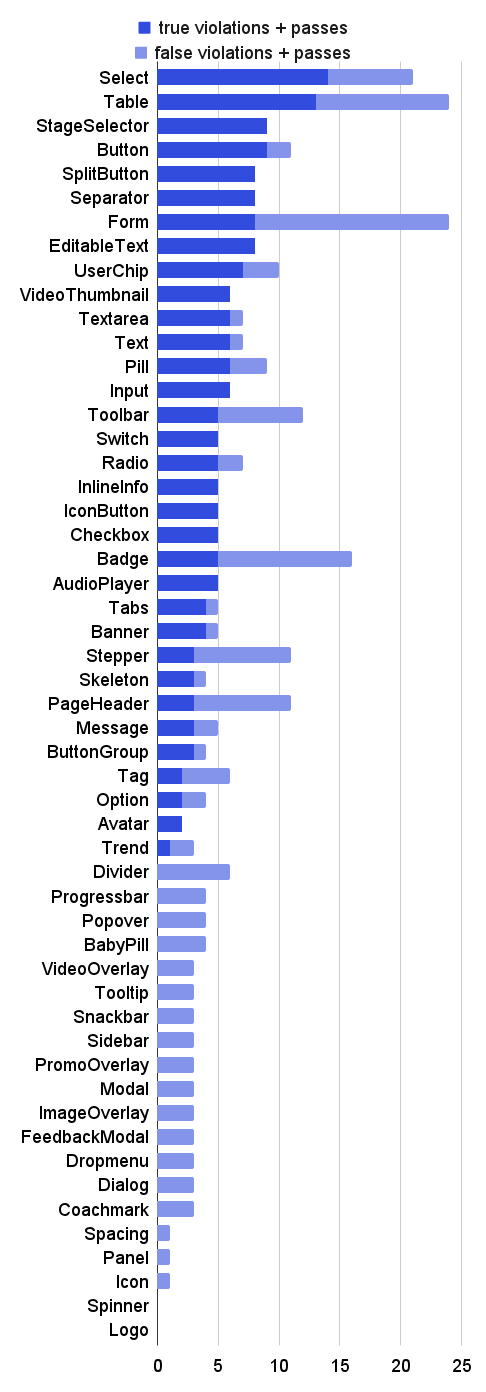
\includegraphics[width=\textwidth]{img/audit-all.png}
	\caption{All issues that were tested by addon-a11y. This means both passed and failed issues combined.}
	\label{fig:audit-all}
\end{figure}

In some cases, there were 0 violations detected, and 0 valid checks passed – this means that the automated testing was not effective (\todo{Make chart or table for this}).

\end{document}